% this file is called up by thesis.tex
% content in this file will be fed into the main document

%: ----------------------- name of chapter  -------------------------
\chapter{Projekt i implementacja} % top level followed by section, subsection


%: ----------------------- paths to graphics ------------------------

% change according to folder and file names
\ifpdf
    \graphicspath{{6/figures/PNG/}{6/figures/PDF/}{6/figures/}}
\else
    \graphicspath{{6/figures/EPS/}{6/figures/}}
\fi

%: ----------------------- contents from here ------------------------

Rozdział ten opisuje architekturę, projekt i implementację przykładowej platformy integracyjnej zwanej dalej SpeechProcessingPlatform, która umożliwi weryfikację proponowanego podejścia. Platforma ta jest projektowana z myślą o architekturze opartej na technologii ESB, którą autorzy uznali za najlepiej nadającą się do realizacji systemów integracyjnych. Rozdział ten zawiera opis najważniejszych części systemu, zależności między nimi oraz format danych wykorzystywanego w komunikacji.

\section{Architektura}

Rysunek \ref{fig:layered_architecture} przedstawia architekturę systemu SpeechProcessingPlatform. Jest ona podzielona na 3 warstwy:

\begin{itemize}
	\item Data Endpoints Layer
	\item Routing Layer
	\item Services Layer
\end{itemize}

\begin{figure}[!h]
	\centering
	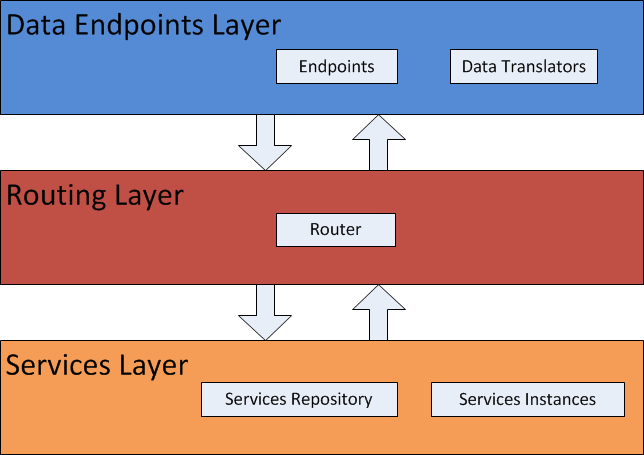
\includegraphics[scale=0.7]{layered_architecture.png}
	\caption{Architektura systemu SpeechProcessingPlatform}\label{fig:layered_architecture}
\end{figure}

Podejście warstwowe ułatwia dekompozycję systemu na niezależne komponenty, które odpowiadają za dobrze zdefiniowany fragment wymaganej funkcjonalności. 
% tu mozna cos dodac jak cos

Warstwa \textit{Data Endpoints Layer} odpowiada za udostępnianie interfejsów dla aplikacji klienckich oraz za transformacje danych do wspólnego formatu. Głównymi elementami tej warstwy są endpointy i translatory danych. Endpointy wystawiają interfejsy umożliwiające dostęp do platformy przy użyciu różnych technologii takich jak REST, FTP, SOAP czy RSS. Zadaniem translatorów jest ujednolicenie danych do postaci używanej w kolejnych warstwach. Dzięki temu komponenty z warstw niższych mają uproszczoną implementację ponieważ skupiają się na obsłudze tylko jednego, dobrze zdefiniowanego formatu. 

Warstwa \textit{Routing Layer} odpowiada za routowanie zadań przetwarzania od endpointów to odpowiednich serwisów, a także za przesyłanie wyników z powrotem do endpointów. Zadania mogą być jedno etapowe jak np. \textit{przetłumacz ten tekst z języka polskiego na język angielski} albo dwu lub więcej etapowe jak np. \textit{rozpoznaj tekst na tym zdjęciu, jeżeli trzeba przetłumacz na język angielski i na jego podstawie wygeneruj dźwięk}.

Głównym elementami ostatniej warstwy, \textit{Services Layer}, jest repozytorium serwisów oraz konkretne ich instancje. Główne zadanie repozytorium to wyszukiwanie i zwracanie odpowiednich instancji w odpowiedzi na żądania warstwy routującej. Najważniejszą cechą wyróżniającą poszczególne serwisy jest typ przetwarzania mowy jaki dostarczają. Ze względu na to kryterium zostały one podzielone na 5 grup, a każda z nich posiada dodatkowe cechy, które także mają wpływ na wynik wyszukiwania:

\begin{itemize}
	\item OCR
	\begin{itemize}
		\item obsługiwane formaty zdjęć
	\end{itemize}
	\item ASR
	\begin{itemize}
		\item obsługiwane języki 
		\item obsługiwane formaty wejściowe
	\end{itemize}
	\item TTS
	\begin{itemize}
		\item obsługiwane języki 
		\item obsługiwane formaty wyjściowe
	\end{itemize}
	\item translacja
	\begin{itemize}
		\item obsługiwane języki
	\end{itemize}
	\item rozpoznawanie języka
\end{itemize}

Oczywiście konkretny serwis może udostępniać więcej niż jeden typ przetwarzania np. serwis translacji może od razu być w stanie rozpoznać język źródłowy, dzięki czemu nie musi mieć tej informacji dostarczonej razem z tekstem.

\begin{figure}[!h]
	\centering
	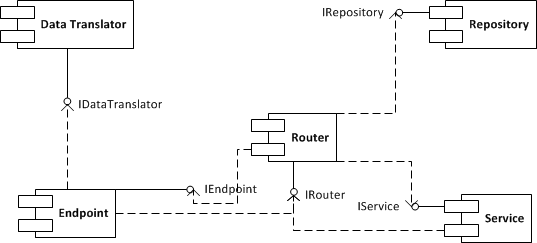
\includegraphics[scale=1.0]{component_uml.png}
	\caption{Diagram komponentów systemu SpeechProcessingPlatform w notacji UML 1.0}\label{fig:component_diagram}
\end{figure}

\section{Projekt}

Jak było wspomniane, do realizacji systemu SpeechProcessingPlatform została wybrana technologia ESB. Głównymi zaletami tej technologii są skalowalność i wysoki poziom abstrakcji, dzięki któremu budowa systemu jest ułatwiona - pozwala skupić się na problemie a nie na szczegółach implementacji. Dodatkowo, kontenery ESB dostarczają dużo użytecznych funkcjonalności takich jak: routing, transformacja danych, komunikacja oparta na wiadomościach, zestaw gotowych endpointów. Wszystko to sprawia, że proces integracji jest znacznie ułatwiony. Projektowanie systemu z użyciem wiadomości jako modelu komunikacji, różni się od tradycyjnego podejścia z blokującymi wywołaniami metod. Interfejsy w postaci listy pól i metod, które dany komponent implementuje zostają zastąpione przez odpowiednie kanały wiadomości oraz format danych, które będą nimi przesyłane. Dzięki użyciu tego modelu, zastosowanie dobrze sprawdzonych wzorców EIP staję się bardzo naturalne. 

\subsection{Warstwa \textit{Data Endpoints Layer}}

Ilustracja \ref{fig:endpoins_layer_project} przedstawia przepływ wiadomości w warstwie \textit{Data Endpoints Layer}. Aplikacje klienckie wysyłają żądanie przetwarzania na określony endpoint, używając wybranego i obsługiwanego przez platformę protokołu. Żądania te zostają przetłumaczone na wspólny format wiadomości używany w dalszych częściach systemu, a następnie przesłane do routera. Dodatkowo, każdy punk końcowy posiada swój indywidualny kanał odpowiedzi, którego adres jest dodawany do wiadomości jako adres zwrotny. Dzięki temu, router będzie wstanie odesłać wynik przetwarzania do odpowiedniego endpointu.

\begin{figure}[!h]
	\centering
	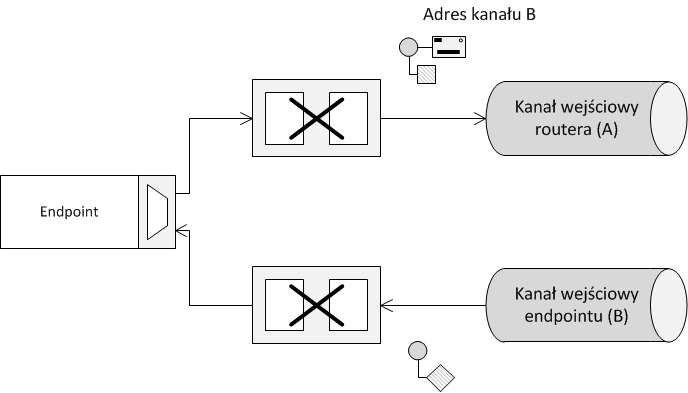
\includegraphics[scale=0.8]{endpoints_layer_flow.png}
	\caption{Diagram przepływu wiadomości w warstwie \textit{Data Endpoints Layer}}\label{fig:endpoins_layer_project}
\end{figure}

Ponieważ przetwarzanie mowy może być procesem czasochłonnym, budowana platforma powinna wspierać komunikację asynchroniczną, która umożliwi uniknięcie zbędnego oczekiwania na odpowiedź. Niektóre punkty końcowe, takie jak FTP czy SMTP są z natury asynchroniczne. Aplikacja wykorzystująca protokół SMTP wysyła emaila z wymaganymi załącznikami na adres endpointa i wraca do swojego przetwarzania. Email zostaje odebrany przez platformę, następuje proces przetwarzania, a odpowiedź jest odsyłana na adres nadawcy. Gdy aplikacja odbierze emaila zwrotnego może zacząć przetwarzanie odpowiedzi w dogodnym dla siebie czasie. Inne końcówki, takie jak REST czy SOAP, posiadają naturę synchroniczną, dlatego aby wspierały one komunikację asynchroniczną należy zastosować dodatkowe mechanizmy. W rozwiązaniu zastosowanym w platformie SpeechProcessingPlatform większość odpowiedzialności za dodanie obsługi asynchronicznej komunikacji spada na kolejne warstwy, dlatego zostanie ono dokładnie opisane w kolejnych podrozdziałach. Jedynym dodatkowym zadaniem punktów końcowych jest oznaczenie wiadomości jako przeznaczonej do przetwarzania asynchronicznego. Reszta procesu, z perspektywy endpointu, nie ulega zmianie. Przy takim oznaczeniu, odpowiedź z warstwy routującej przychodzi bardzo szybko, lecz zawiera ona tylko identyfikator odpowiedzi, dzięki któremu aplikacja kliencka będzie mogła odpytać system czy jej zadanie zostało już zakończone. Takie zapytanie jest traktowane w taki sam sposób jak żądanie przetwarzania. Jeżeli zadanie zostało zakończone, wynik zostanie zwrócony aplikacji. Jeżeli nie, aplikacja będzie musiała wykonać zapytanie ponownie.

\subsection{Warstwa \textit{Routing Layer}}

\subsubsection{Przepływ regularnych wiadomości}
Diagram \ref{fig:routing_layer_project} przedstawia, przepływ wiadomości, które zostały wysłane na adres warstwy routującej. Żadania, które już wcześniej były poddane transformacji, są gotowe aby wysłać je do odpowiednich serwisów. Komponent routujący, nie posiada stałych, wyznaczonych tras, lecz wybiera je za każdym razem gdy otrzyma wiadomość na swój kanał wejściowy. Jeżeli zadanie zostanie uznane za zakończone zostaje ono wysłane z powrotem do odpowiedniego endpointu na podstawie adresu zwrotnego. Jeżeli do zakończenia zadania potrzebny jest jeszcze jakiś etap przetwarzania, router wykonuje zapytanie do rejestru serwisów w celu uzyskania adresu serwisu spełniającego wymagania zadania. Jeżeli zostanie znaleziony odpowiedni serwis , żądanie przetwarzania zostaje opakowane w w dodatkową kopertę, której adres zwrotny wskazuje na kanał wejściowy routera. Tak przygotowana wiadomość zostaje wysłana na adres uzyskany od rejestru serwisów. Po przetworzeniu, wiadomość jest odsyłana na adres wejściowy routera i jest podawana procesowi routowania ponownie. Jeżeli repozytorium nie zawiera serwisu spełniającego wymagania zadania, wiadomość jest odsyłana z powrotem do endpointu z odpowiednim kodem błędu. 

\begin{figure}[!h]
	\centering
	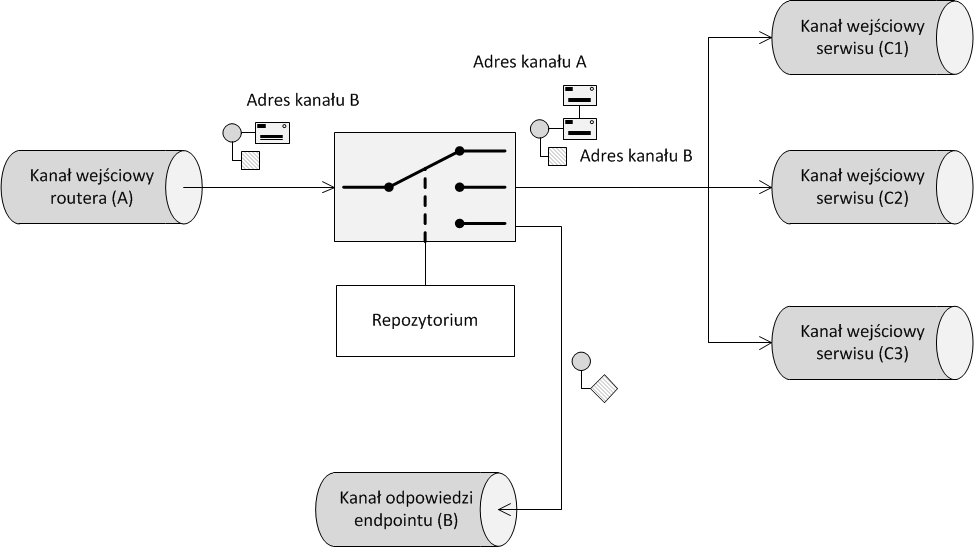
\includegraphics[scale=0.55]{router_flow.png}
	\caption{Diagram przepływu wiadomości w warstwie \textit{Routing Layer}}\label{fig:routing_layer_project}
\end{figure}

\begin{figure}[!h]
	\centering
	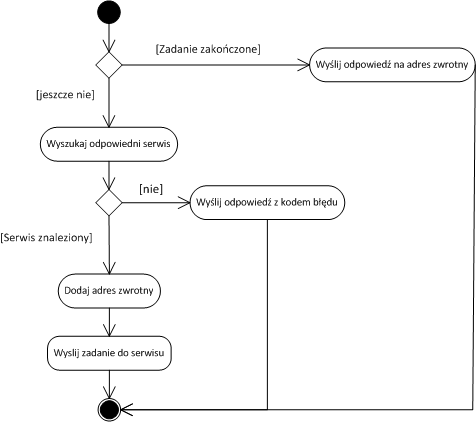
\includegraphics[scale=1.0]{router_activity.png}
	\caption{Diagram czynności komponentu routującego. }\label{fig:router_activity_diagram}
\end{figure}

\subsubsection{Przepływ wiadomości asynchronicznych}
W celu obsługi wiadomości w sposób asynchroniczny, jeżeli wykorzystywany endpoint nie zapewnia wparcia dla takiej komunikacji, należy poprzedzić proces routowania dodatkowymi krokami.
Diagram \ref{fig:asynchronous_detour} przedstawia rozwiązanie zastosowane w SpeechProcessingPlatform. Ważnym aspektem w prezentowanej koncepcji jest wprowadzenie dodatkowego typu serwisów, których zadaniem jest przechowywanie odpowiedzi pod odpowiednim kluczem. Serwisy w dalszej części pracy będą zwane serwisami storage. Pierwszym etapem jest rozdzielenie wiadomości na dwie grupy synchroniczne i asynchroniczne. Podział ten jest dokonywany na podstawie oznaczenia wykonanego przez endpoint zlecający, a także na podstawie obecności chociaż jednego serwisu storage. Jeżeli chociaż jeden z tych warunków nie jest spełniony żądanie będzie obsłużony w sposób opisany w poprzednim podrozdziale. Jeżeli oby dwa warunki są spełnione wiadomość jest poddawana kilku dodatkowym operacjom przed wysłaniem jej do routera. Pierwsza z nich to usunięcie oznaczenia do przetwarzania asynchronicznego. Druga to wygenerowanie i dodanie do wiadomości unikalnego identyfikatora, który posłuży jako klucz przy przechowywaniu docelowej odpowiedzi. Następnym krokiem jest wygenerowanie zastępczej odpowiedzi i wysłanie jej do endpointu. Odpowiedz ta zawiera wygenerowany wcześniej identyfikator, co pozwoli aplikacji klienckiej odpytanie systemu o odpowiedz na oryginalne zadanie. Ostatnim krokiem jest podmiana adresu zwrotnego w oryginalnej wiadomości na adres serwisu storage. Dalsze przetwarzanie wygląda tak samo jak w wypadku wiadomości synchronicznych.


 % mozna dodać obrazek do correlation idetifier po słowach : ...nagłówki: unikalny idetyfikator, oraz....

\begin{figure}[!h]
	\centering
	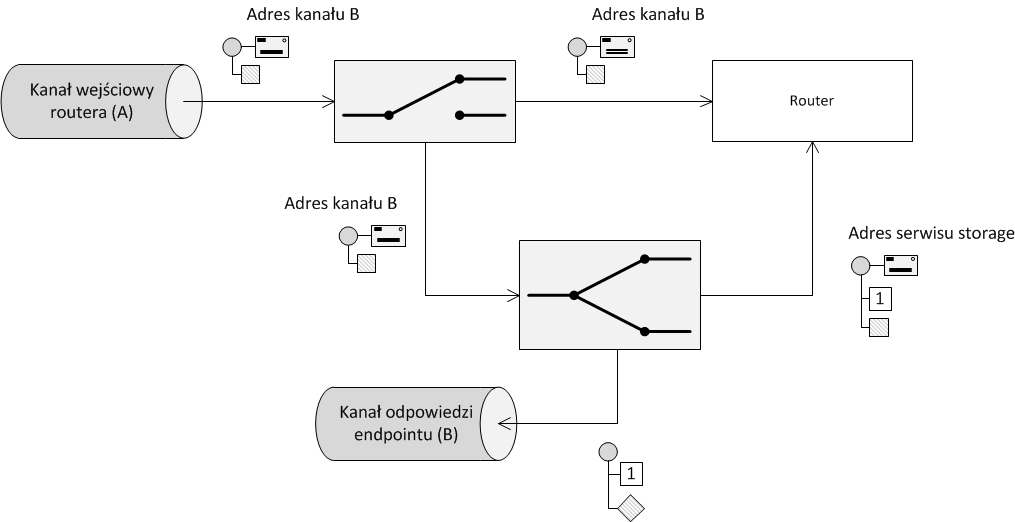
\includegraphics[scale=0.55]{asynchronous_detour.png}
	\caption{Diagram przepływu dla komunikacji asynchronicznej}\label{fig:asynchronous_detour}
\end{figure}

\begin{figure}[!h]
	\centering
	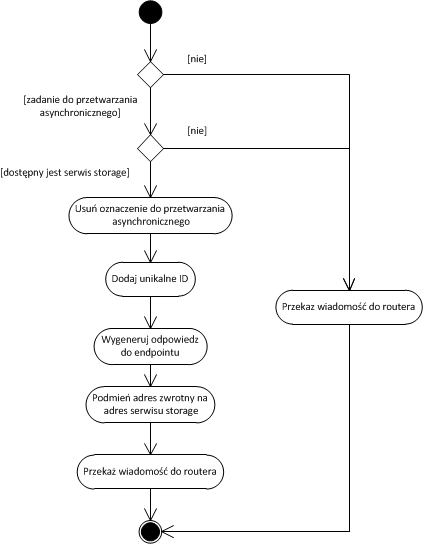
\includegraphics[scale=1.0]{asynchronous_activity_uml.png}
	\caption{Diagram czynności dla wiadomości asynchronicznych. }\label{fig:asynchronous_activity}
\end{figure}

\subsection{Warstwa \textit{Services Layer}}

Pierwszym komponentem z warstwy \textit{Services Layer}, który bierze udział podczas przetwarzania wiadomości jest repozytorium serwisów. Można byłoby obejść się bez tego komponentu, lecz wtedy wymagałoby to zapisania gdzieś w implementacji warstwy \textit{Routing Layer} stałych ścieżek lub zestawu reguł na podstawie których podejmowana byłaby decyzja o dalszej trasie wiadomości. Takie podejście mocno związałoby platformę z konkretnymi serwisami, dodanie nowego serwisu wiązało by się ze zmianą implementacji. Dzięki zastosowaniu repozytorium, które wprowadza dodatkową warstwę abstrakcji nad konkretnymi serwisami syntezy mowy, całość systemu nie jest związana z konkretnym dostawcą usług syntezy. Dodatkowym plusem takiego rozwiązania jest możliwość dynamicznego wyboru serwisów w zależności od zmieniających się warunków zewnętrznych. Platformę można rozszerzyć o komponenty monitorujące zachowanie się serwisów w czasie rzeczywistym co pozwoli na wybór najlepszej instancji w danym momencie. 
Aby nie wiązać platformy z konkretną implementacją repozytorium został wprowadzony interfejs, który musi być zaimplementowany przez komponenty chcące pełnić role repozytorium serwisów. Takie podejście pozwoli na użycie różnych implementacji opartych na różnych technologiach np Spring czy OSGI. Fragment kodu \ref{lst:repository_interface} przedstawia omawiany interfejs:

\lstset{language=Java, tabsize=4, caption=Definicja interfejsu ISreviceRepository w języku Java.,label=lst:repository_interface}

\begin{center}
\begin{lstlisting}
public interface SreviceRepository {
	Collection<String> lookupServices(Class type);
	Collection<String> lookupServices(Class type, Map<String, String> metaData);
	String lookupService(Class type);
	String lookupService(Class type, Map<String, String> metaData);
}
\end{lstlisting}
\end{center}

Chociaż repozytorium serwisów jest ważnym komponentem to nie bierze ono czynnego udziału w przetwarzaniu wiadomości. Adres serwisu który zostaje zwrócony jako odpowiedź na żądanie routera służy do wysłania zadania do odpowiedniej instancji serwisu. Diagram \ref{fig:services_layer_project} przedstawia przepływ wiadomości w warstwie \textit{Services Layer}. Przepływ ten jest stosunkowo prosty. Wiadomości pojawiające się w kanale wejściowym są odbierane i poddawane przetwarzaniu. Odpowiedź odsyłana jest na adres zwrotny zawarty w wiadomości, który zawsze wskazuję na adres kanału wejściowego routera. 

\begin{figure}[!h]
	\centering
	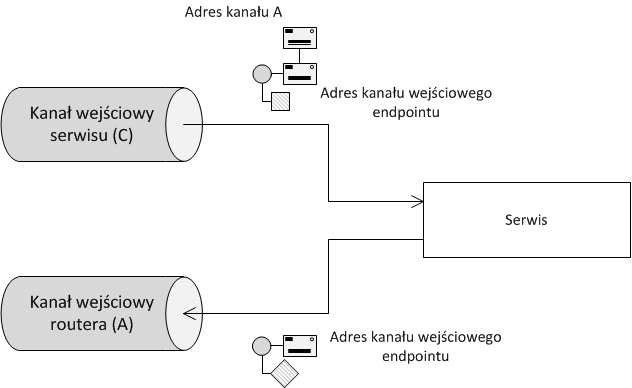
\includegraphics[scale=0.85]{services_layer_flow.png}
	\caption{Diagram przepływu wiadomości w warstwie \textit{Services Layer}}\label{fig:services_layer_project}
\end{figure}

Pierwszym wymaganiem stawianym konkretnym instancjom serwisów jest implementacja interfejsu \textit{IMessageEnabledService} \ref{lst:service_interface}. Interfejs ten posiada tylko jedną metodę, która zwraca adres kanału wejściowego danego serwisu. Spełnienie tego wymagania jest konieczne aby repozytorium było w stanie odnaleźć serwis i zwrócić jego adres routerowi, jednak aby dana instancja pełniła jakąkolwiek rolę w systemie musi także udostępniać informację o funkcjonalności przez niej dostarczanej. W tym celu instancje muszą implementować dodatkowe interfejsy, które jednoznacznie określają udostępnianą funkcjonalność. Ponieważ komunikacją między serwisami a resztą systemu odbywa się przez kanały wiadomości, interfejsy te służą tylko do oznaczenia serwisów a nie jako kontrakt miedzy nimi a, komponentami z nich korzystającymi. Takie użycie interfejsu jest znane jako wzorzec \textit{Marker interface} \cite{bloch2008}.

\lstset{language=Java, tabsize=4, caption=Definicja interfejsu IMessageEnabledService w języku Java.,label=lst:service_interface}

\begin{center}
\begin{lstlisting}
public interface MessageEnabledService {
	String getServiceURI();
}
\end{lstlisting}
\end{center}

Jak było wspomniane wcześniej serwisy syntezy mowy zostały podzielone na 5 podstawowych grup, lecz nic nie stoi na przeszkodzie aby dodać kolejne, tak jak to ma miejsce z serwisami typu storage. Jedyne co trzeba zrobić to zarejestrować serwis pod odpowiednim interfejsem. Fragment kodu \ref{lst:services_interfaces} przedstawia 5 interfejsów syntezy mowy plus interfejs serwisu storage.

\lstset{language=Java, tabsize=4, caption=Definicja interfejsów serwisów w języku Java.,label=lst:services_interfaces}

\begin{center}
\begin{lstlisting}

public interface OCRService {
}

public interface TTSService {
}

public interface ASRService {
}

public interface TranslationService {
}

public interface LanguageRecognitionService {
}

public interface StorageService {
}
\end{lstlisting}
\end{center}

Drugim i ostatnim wymaganiem stawianym przed implementacjami serwisów jest obsługa wiadomości w w wewnętrznym formacie używanym w systemie. Jest to spowodowane brakiem informacji na temat jaki format wiadomości jest obsługiwany przez dany serwis. Podczas routowania wiadomości znany jest tylko adres i typ docelowego serwisu, dlatego router nie jest w stanie przetransformować wiadomości do obsługiwanego formatu. 


Większość dostępnych serwisów syntezy mowy nie była tworzona z myślą o obsłudze komunikacji opartej na wiadomościach, a nawet jeśli,  to na pewno nie obsługują one formatu budowanego systemu. Aby możliwe było użycie gotowych serwisów w budowanym systemie użyć komponentów które będą działać na zasadzie proxy i to te komponenty będą rejestrować sie w rejestrze serwisów. Po otrzymaniu wiadomości komponent proxy, podda ją wymaganej transformacji po czym wyśle zadanie do konkretnej instancji serwisu, używając przy tym odpowiedniego adaptera, jeżeli zajdzie taka potrzeba. 

\begin{figure}[!h]
	\centering
	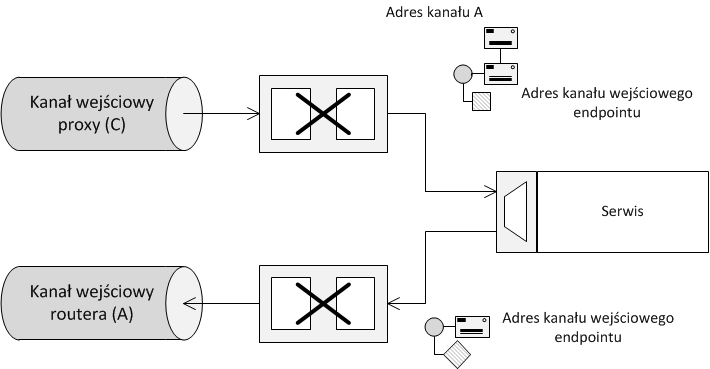
\includegraphics[scale=0.8]{proxy_layer_flow.png}
	\caption{Proxy wraz z elementami transformującymi oraz adapterem. }\label{fig:servis_proxy.}
\end{figure}






\section*{Podsumowanie} 


% można wrzucic obrazek całego systemu

%Jednym z rozwiązań jest użycie wzorca \textit{Correlation Identifier}\cite{eaipatterns}:

%\begin{figure}[!h]
%	\centering
%	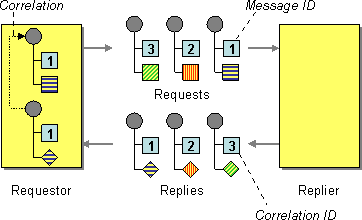
\includegraphics{CorrelationIdentifierSolution.png}
%	\caption{Wzorzec \textit{Correlation Identifier}: \url{http://www.eaipatterns.com/img/CorrelationIdentifierSolution.gif}}\label{fig:correlation_identifier}
%\end{figure}

%Endpoint po otrzymaniu żądania generuje dla niego unikalny identyfikator, który odsyła aplikacji nie czekając na wynik przetwarzania. Ten sam identyfikator jest dodawany do wiadomości %wysyłanej do routera, lecz tym razem adres zwrotny wskazuje nie na endpoint lecz na serwis 



% rysunek z podziałęm na komponenty,
% rysunek EIP - ale to może być już w projekcie.
% proekt, interfejsy, chierarchie klas. 









% ---------------------------------------------------------------------------
%: ----------------------- end of thesis sub-document ------------------------
% ---------------------------------------------------------------------------

